%==========================================================================
\chapter{Structured-Grid Interface}
\label{Structured-Grid Interface}

In order to get access to the most efficient and scalable solvers for
structured-grid applications, users should use the \code{Struct}
interface described in this chapter.  This interface will also provide
access (this is not yet supported) to solvers in \hypre{} that were
designed for unstructured-grid applications and sparse linear systems
in general.  These additional solvers are usually provided via the
unstructured-grid interface (\code{FEI}) or the linear-algebraic
interface (\code{IJ}) described in Chapters \ref{chapter-FEI} and
\ref{chapter-IJ}.

Figure \ref{fig-fv-grid} gives an example of the type of grid
currently supported by the \code{Struct} interface.
\begin{figure}
\centering
\includegraphics[width=4in]{fv_grid.eps}
\caption{%
An example 2D finite-volume grid, distributed accross two processors.}
\label{fig-fv-grid}
\end{figure}
The interface uses a finite-difference or finite-volume style, and
currently supports only scalar PDEs (i.e., one unknown per gridpoint).
There is an effort to extend it to use a finite-element style (similar
to the \code{FEI}, but on structured grids), and to support PDE systems.

There are four basic steps involved in setting up the linear system
to be solved:
\begin{itemize}
\item set up the grid,
\item set up the stencil,
\item set up the matrix,
\item set up the right-hand-side.
\end{itemize}
To describe each of these steps in more detail, consider solving the
2D Laplacian problem
\begin{equation}\label{eqn-laplacian}
\left \{
\begin{array}{ll}
\nabla^2 u = f , & \mbox{in the domain}, \\
u = 0,           & \mbox{on the boundary}.
\end{array}
\right .
\end{equation}
Assume (\ref{eqn-laplacian}) is discretized using standard 5-pt
finite-volumes on the uniform grid pictured in \ref{fig-fv-grid}, and
assume that the problem data is distributed across two processes as
depicted.

%==========================================================================

\section{Setting Up the Grid}
\label{Setting Up the Grid}

The grid is described via a global {\em index space}, i.e., via
integer tuples (triples in 3D).  The integers may have any value,
negative or positive.  The global indexes allow \hypre{} to discern
how data is related spatially, and how it is distributed across the
parallel machine.

Each process describes that portion of the grid that it ``owns'', one
{\em box} at a time.  For example, in the figure, the global grid can
be described in terms of three boxes, two owned by process 0, and one
owned by process 1.  A box is described in terms of a lower and upper
index.  On process 0, the following code will set up the grid shown in
the figure (code for process 1 is similar).
\begin{display}
\begin{verbatim}

HYPRE_StructGrid  grid;

int               ilower[2][2] = {{-3, 1}, {0, 1}};
int               iupper[2][2] = {{-1, 2}, {2, 4}};

HYPRE_StructGridCreate(MPI_COMM_WORLD, 2, &grid);

HYPRE_StructGridSetExtents(grid, ilower[0], iupper[0]);
HYPRE_StructGridSetExtents(grid, ilower[1], iupper[1]);

HYPRE_StructGridAssemble(grid);

\end{verbatim}
\end{display}

The \code{HYPRE_StructGridCreate()} routine creates an empty 2D grid
object that lives on the \code{MPI_COMM_WORLD} communicator.  The
\code{HYPRE_StructGridSetExtents()} routine adds a new box to the grid.
The \code{HYPRE_StructGridAssemble()} routine is a collective call
(i.e., must be called on all processes), and finalizes the grid
assembly, making the grid ``ready for use'' elsewhere.

%==========================================================================

\section{Setting Up the Stencil}
\label{Setting Up the Stencil}

Here is the 5-pt stencil description
\begin{equation}\label{eqn-stencil-description}
\left [
\begin{array}{ccc}
        & ( 0, 1) &         \\
(-1, 0) & ( 0, 0) & ( 1, 0) \\
        & ( 0,-1) &        
\end{array}
\right ]
\equiv
\left [
\begin{array}{ccc}
    & S_4 &     \\
S_1 & S_0 & S_2 \\
    & S_3 &    
\end{array}
\right ] .
\end{equation}
On process 0, the following code will set up the stencil in
(\ref{eqn-stencil-description}).
\begin{display}
\begin{verbatim}

HYPRE_StructStencil  stencil;
int                  offsets[5][2] = {{0,0}, {-1,0}, {1,0}, {0,-1}, {0,1}};
int                  s;

HYPRE_StructStencilCreate(2, 5, &stencil);

for (s = 0; s < 5; s++)
{
   HYPRE_StructStencilSetElement(stencil, s, offsets[s]);
}

\end{verbatim}
\end{display}

%==========================================================================

\section{Setting Up the Matrix}
\label{Setting Up the Matrix}

Here is the 5-pt stencil for the Laplacian
\begin{equation}\label{eqn-stencil-laplacian}
\left [
\begin{array}{ccc}
   & -1 &    \\
-1 &  4 & -1 \\
   & -1 &   
\end{array}
\right ] .
\end{equation}
On process 0, the following code will set up matrix values associated
with the center ($S_0$) and south ($S_3$) stencil entries in
(\ref{eqn-stencil-description}) / (\ref{eqn-stencil-laplacian}).
\begin{display}
\begin{verbatim}

HYPRE_StructMatrix  A;
double              values[24];
int                 stencil_indices[2] = {0,3};
int                 i;

HYPRE_StructMatrixCreate(MPI_COMM_WORLD, grid, stencil, &A);
HYPRE_StructMatrixInitialize(A);

for (i = 0; i < 24; i += 2)
{
   values[i]   =  4.0;
   values[i+1] = -1.0;
}

HYPRE_StructMatrixSetBoxValues(A, ilower[0], iupper[0], 2,
                               stencil_indices, values);
HYPRE_StructMatrixSetBoxValues(A, ilower[1], iupper[1], 2,
                               stencil_indices, values);

HYPRE_StructMatrixAssemble(A);

\end{verbatim}
\end{display}

%==========================================================================

\section{Setting Up the Right-Hand-Side}
\label{Setting Up the Right-Hand-Side}

On process 0, the following code will set up right-hand-side.
\begin{display}
\begin{verbatim}

HYPRE_StructVector  b;
double              values[12];
int                 i;

HYPRE_StructVectorCreate(MPI_COMM_WORLD, grid, stencil, &b);
HYPRE_StructVectorInitialize(b);

for (i = 0; i < 12; i++)
{
   values[i]   =  0.0;
}

HYPRE_StructVectorSetBoxValues(b, ilower[0], iupper[0], values);
HYPRE_StructVectorSetBoxValues(b, ilower[1], iupper[1], values);

HYPRE_StructVectorAssemble(b);

\end{verbatim}
\end{display}

%==========================================================================

